\section{Parameters schrijven}

Momenteel is het programma die op de testkast staat alleen werkend bij één type motor namelijk de OEMER HQL100X. Er is wel een knop waar “Write motor parameters” op staat maar deze knop werkt in werkelijkheid nog niet. Het programma heeft één parameter set voor de motor en kan niet wisselen tussen parametersets. Het programma ziet er uit als in figuur \ref{fig:TestProgrammaVoorheen}. De motor kan worden bestuurd doormiddel van de slidebar naar de gewenste motorsnelheid. Er is verder nog geen testprocedure er wordt alleen gekeken naar of de motor werkt en of de motor niet te veel trilt.

\begin{figure}[H]
	\centering
	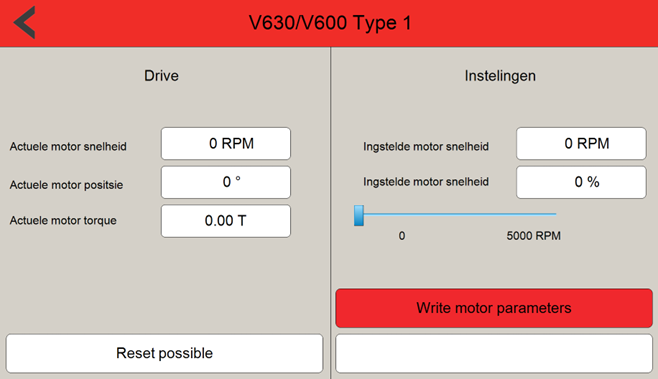
\includegraphics[width=350pt]{TestProgrammaVoorheen}
	\label{fig:TestProgrammaVoorheen}
	\caption{Programma op testkast}
\end{figure}

\subsection{Parameters automatisch inladen}

Parameters moeten worden geschreven met \gls{SoE} (\gls{SERCOS} over \gls{EtherCAT}). Beckhoff biedt hier een aantal bruikbare functieblokken voor aan in \gls{TwinCAT} genaamd FB\_SoERead en FB\_SoEWrite in de Tc2\_MC2\_Drive library. Een voorbeeld flowchart over hoe dit zou kunnen werken ziet er als volgt uit:

\begin{figure}[H]
	\centering
	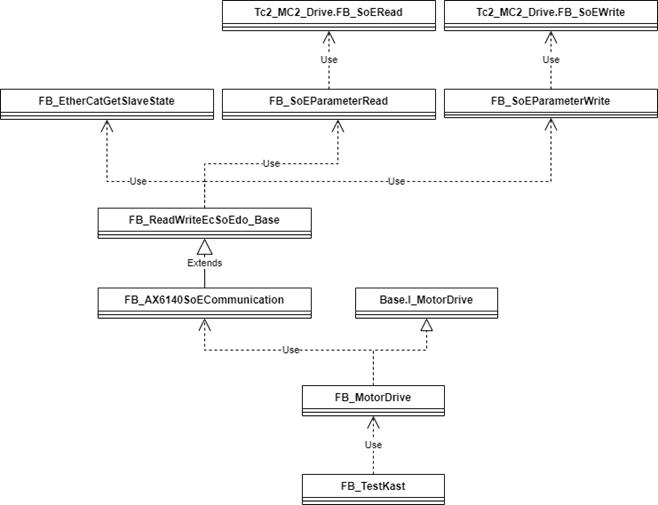
\includegraphics[width=\linewidth]{SoEReadWrite}
	\label{fig:SoEReadWrite}
	\caption{SoE Read write met TwinCAT}
\end{figure}

In figuur \ref{fig:SoEReadWrite} is gedacht aan herbruikbaarheid daarom is zo veel mogelijk standaard communicatie functionaliteit geïmplementeerd in FB\_ReadWriteEcSoEdo\_Base zodat in FB\_AX6140SoECommunication alleen de drive specifieke dingen geregeld hoeven te worden. Vervolgens kan de motordrive dit communicatie FB gemakkelijk gebruiken om informatie over en weer te sturen.

\begin{figure}[H]
	\centering
	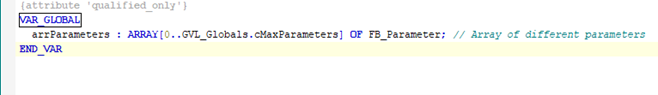
\includegraphics[width=\linewidth]{ParameterArray}
	\label{fig:ParameterArray}
	\caption{Parameter Array}
\end{figure}

Om alle parameter informatie makkelijk te kunnen uitlezen over \gls{ADS} is er een array gemaakt van FB\_Parameter. De parameter heeft bijvoorbeeld een buffer, \gls{IDN} en een counter zodat de FB\_AX5140SoECommunication weet hoe vaak de parameter per seconde uit gelezen moet worden.

\begin{figure}[H]
	\centering
	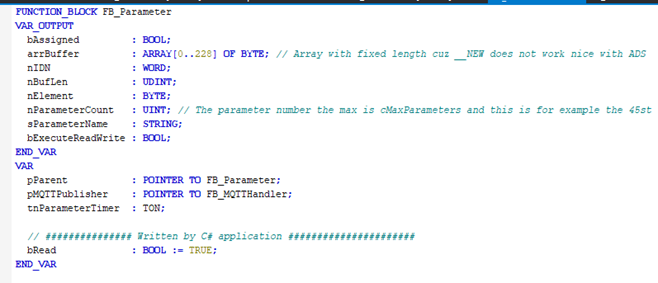
\includegraphics[width=\linewidth]{FB_Parameter}
	\label{fig:FB_Parameter}
	\caption{FB\_Parameter}
\end{figure}

Helaas bleek het slecht mogelijk om dynamisch geheugen toe te wijzen aan de buffer omdat de pointer die hieruit komt slecht uit te lezen is over \gls{ADS} in de C\# applicatie. Voortman zelf gebruikt ook geen dynamisch geheugen in hun \gls{PLC} code. Daarom is ervoor gekozen om een byte array te gebruiken die altijd groot genoeg is voor de data van de parameter.

\vspace{0.5cm}

Daarnaast heeft elke parameter ook een pointer naar een \gls{MQTT} handler om eventueel de parameter ook te publiceren waardoor er ook op afstand mee gekeken kan worden.

\vspace{0.5cm}

In de \gls{gui} kan bijvoorbeeld een parameter aangemaakt worden er komt dan een scherm tevoorschijn waar men kan kiezen welke parameter er op het scherm gemonitord moet worden. Dit is te zien in figuur \ref{fig:GUIParameter}. In figuur \ref{fig:ParameterMonitor} is te zien dat er een grafiek is aangemaakt voor de parameter die de parameter zal monitoren. De \gls{PLC} en de \gls{gui} moeten kunnen communiceren met elkaar dit proces is afgebeeld in figuur \ref{fig:CommunicatieGUIenPLC}.

\begin{figure}[H]
	\centering
	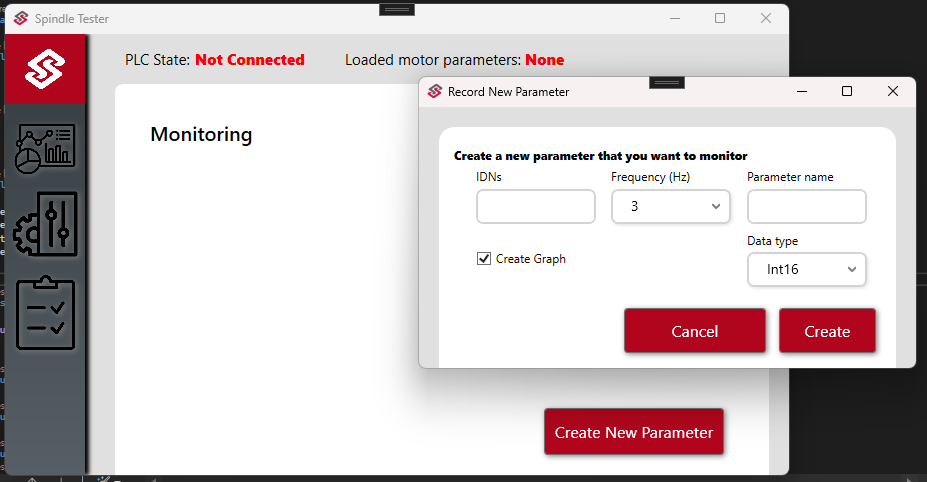
\includegraphics[width=\linewidth]{GUIParameter}
	\label{fig:GUIParameter}
	\caption{Parameter aanmaken om uit te lezen}
\end{figure}

\begin{figure}[H]
	\centering
	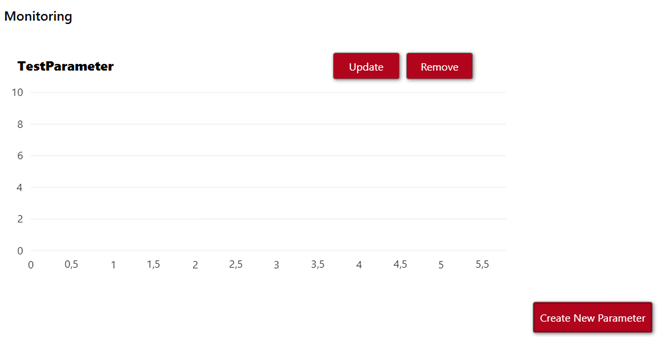
\includegraphics[width=\linewidth]{ParameterMonitor}
	\label{fig:ParameterMonitor}
	\caption{Grafiek van de parameter}
\end{figure}

\begin{figure}[H]
	\centering
	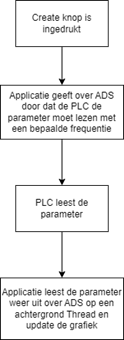
\includegraphics[width=90pt]{CommunicatieGUIenPLC}
	\label{fig:CommunicatieGUIenPLC}
	\caption{Communicatie PLC en GUI}
\end{figure}

\begin{figure}[H]
	\centering
	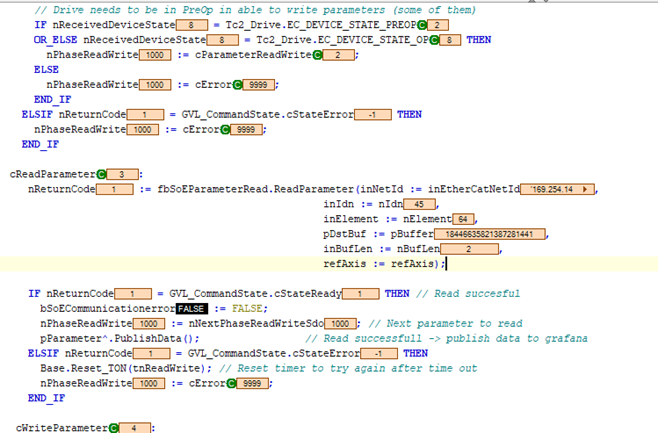
\includegraphics[width=\linewidth]{ParameterReading}
	\label{fig:ParameterRead}
	\caption{S\_0\_0045 wordt uitgelezen uit de drive door de \gls{PLC}}
\end{figure}

